% This is "sig-alternate.tex" V2.0 May 2012
% This file should be compiled with V2.5 of "sig-alternate.cls" May 2012
%
% This example file demonstrates the use of the 'sig-alternate.cls'
% V2.5 LaTeX2e document class file. It is for those submitting
% articles to ACM Conference Proceedings WHO DO NOT WISH TO
% STRICTLY ADHERE TO THE SIGS (PUBS-BOARD-ENDORSED) STYLE.
% The 'sig-alternate.cls' file will produce a similar-looking,
% albeit, 'tighter' paper resulting in, invariably, fewer pages.
%
% ----------------------------------------------------------------------------------------------------------------
% This .tex file (and associated .cls V2.5) produces:
%       1) The Permission Statement
%       2) The Conference (location) Info information
%       3) The Copyright Line with ACM data
%       4) NO page numbers
%
% as against the acm_proc_article-sp.cls file which
% DOES NOT produce 1) thru' 3) above.
%
% Using 'sig-alternate.cls' you have control, however, from within
% the source .tex file, over both the CopyrightYear
% (defaulted to 200X) and the ACM Copyright Data
% (defaulted to X-XXXXX-XX-X/XX/XX).
% e.g.
% \CopyrightYear{2007} will cause 2007 to appear in the copyright line.
% \crdata{0-12345-67-8/90/12} will cause 0-12345-67-8/90/12 to appear in the copyright line.
%
% ---------------------------------------------------------------------------------------------------------------
% This .tex source is an example which *does* use
% the .bib file (from which the .bbl file % is produced).
% REMEMBER HOWEVER: After having produced the .bbl file,
% and prior to final submission, you *NEED* to 'insert'
% your .bbl file into your source .tex file so as to provide
% ONE 'self-contained' source file.
%
% ================= IF YOU HAVE QUESTIONS =======================
% Questions regarding the SIGS styles, SIGS policies and
% procedures, Conferences etc. should be sent to
% Adrienne Griscti (griscti@acm.org)
%
% Technical questions _only_ to
% Gerald Murray (murray@hq.acm.org)
% ===============================================================
%
% For tracking purposes - this is V2.0 - May 2012

\documentclass{sig-alternate}
\usepackage{graphicx} %package to manage images
\usepackage{fixltx2e} %package for subscripts because latex is retarded
\usepackage [english]{babel}
\usepackage [autostyle, english = american]{csquotes}
\MakeOuterQuote{"} %package for quotes because latex is, you guessed it, retarded
\begin{document}
%
% --- Author Metadata here ---
%\conferenceinfo{WOODSTOCK}{'97 El Paso, Texas USA}
\CopyrightYear{2015} % Allows default copyright year (20XX) to be over-ridden - IF NEED BE.
\crdata{???}  % Allows default copyright data (0-89791-88-6/97/05) to be over-ridden - IF NEED BE.
% --- End of Author Metadata ---

\title{Modeling Traffic in New York to Determine Optimal Taxi Routes}
%Format\titlenote{(Produces the permission block, and
%copyright information). For use with
%SIG-ALTERNATE.CLS. Supported by ACM.}}
%\subtitle{[Extended Abstract]
%\titlenote{A full version of this paper is available as
%\textit{Author's Guide to Preparing ACM SIG Proceedings Using
%\LaTeX$2_\epsilon$\ and BibTeX} at
%\texttt{www.acm.org/eaddress.htm}}}
%
% You need the command \numberofauthors to handle the 'placement
% and alignment' of the authors beneath the title.
%
% For aesthetic reasons, we recommend 'three authors at a time'
% i.e. three 'name/affiliation blocks' be placed beneath the title.
%
% NOTE: You are NOT restricted in how many 'rows' of
% "name/affiliations" may appear. We just ask that you restrict
% the number of 'columns' to three.
%
% Because of the available 'opening page real-estate'
% we ask you to refrain from putting more than six authors
% (two rows with three columns) beneath the article title.
% More than six makes the first-page appear very cluttered indeed.
%
% Use the \alignauthor commands to handle the names
% and affiliations for an 'aesthetic maximum' of six authors.
% Add names, affiliations, addresses for
% the seventh etc. author(s) as the argument for the
% \additionalauthors command.
% These 'additional authors' will be output/set for you
% without further effort on your part as the last section in
% the body of your article BEFORE References or any Appendices.

\numberofauthors{2} %  in this sample file, there are a *total*
% of EIGHT authors. SIX appear on the 'first-page' (for formatting
% reasons) and the remaining two appear in the \additionalauthors section.
%
\author{
% You can go ahead and credit any number of authors here,
% e.g. one 'row of three' or two rows (consisting of one row of three
% and a second row of one, two or three).
%
% The command \alignauthor (no curly braces needed) should
% precede each author name, affiliation/snail-mail address and
% e-mail address. Additionally, tag each line of
% affiliation/address with \affaddr, and tag the
% e-mail address with \email.
%
% 1st. author
\alignauthor
Pranav Batra\\
       \affaddr{Vanderbilt University}\\
       \affaddr{Nashville, TN 37235, USA}\\
       \email{pranav.batra@vanderbilt.edu}
% 2nd. author
\alignauthor
Ethan Dixius\\
       \affaddr{Vanderbilt University}\\
       \affaddr{Nashville, TN 37235, USA}\\
       \email{ethan.dixius@vanderbilt.edu}
% 3rd. author
%\alignauthor
%Ian Simonson\\
%       \affaddr{Vanderbilt University}\\
%       \affaddr{Nashville, TN 37235, USA}\\
%       \email{ian.simonson@vanderbilt.edu}
}

\maketitle
\begin{abstract}
A model predicting the traffic speed on each road in New York at each hour of the day will be constructed based on New York taxi data from 2013. This model will be used to estimate trip times and determine if taxi drivers are overcharging passengers. Thus far, a model for traffic flow based on historical traffic volume data from 2001-2011 has been constructed. This model will be used to validate the traffic speed model in accordance with Greenshields' model.
\end{abstract}

% A category with the (minimum) three required fields
%\category{H.4}{Information Systems Applications}{Miscellaneous}
%A category including the fourth, optional field follows...
%\category{D.2.8}{Software Engineering}{Metrics}[complexity measures, performance measures]

%\terms{Theory}

%\keywords{ACM proceedings, \LaTeX, text tagging}

\section{Introduction}
Taxis are a widely used form of transportation, especially in large cities such as New York. However, it is often difficult to tell how long a taxi ride will take given the traffic conditions and how much the fare will be. To this end, we plan to develop an Android application that can estimate the expected time for a taxi ride based on historical data. While developing this application, we will also investigate how often taxi drivers take suboptimal routes to increase fares, thereby overcharging passengers. Thus far, Perl scripts have been written for preliminary analysis of the historical taxi and traffic volume data.

\section{Model}
There are three main components to the prediction algorithm for taxi trip times. First, a model for the traffic speed on each road at each hour of the day will be constructed based on taxi data from 2013. Next, a directed graph containing the roads in New York will be constructed. The graph is directed since the traffic in each direction often differs substantially. Each intersection will be a vertex on the graph (specified by latitude, longitude); each edge will contain the distance of the corresponding road segment along with the direction (specified by FHWA, the Federal Highway Administration). This graph will be used both for the construction of the traffic speed model and to determine the optimal route between any two points on the graph at any time of day, given the traffic speed model (via an A* search, with Manhattan distance as the heuristic). Finally, the taxi data will be reanalyzed using the road graph and traffic speed model to determine if taxi drivers are overcharging or taking suboptimal routes to increase fares.

\subsection{Traffic flow}
The model for traffic speed will be validated against traffic flow data (2001-2011) via Greenshields' model\cite{green}. Greenshields' model (Fig. 1) relates traffic flow to traffic speed as follows:
\begin{equation}q=\frac{(A-v)\times v}{B}\end{equation}
where q is the flow, v is the speed, and A and B are constants.

\begin{figure}
\centering
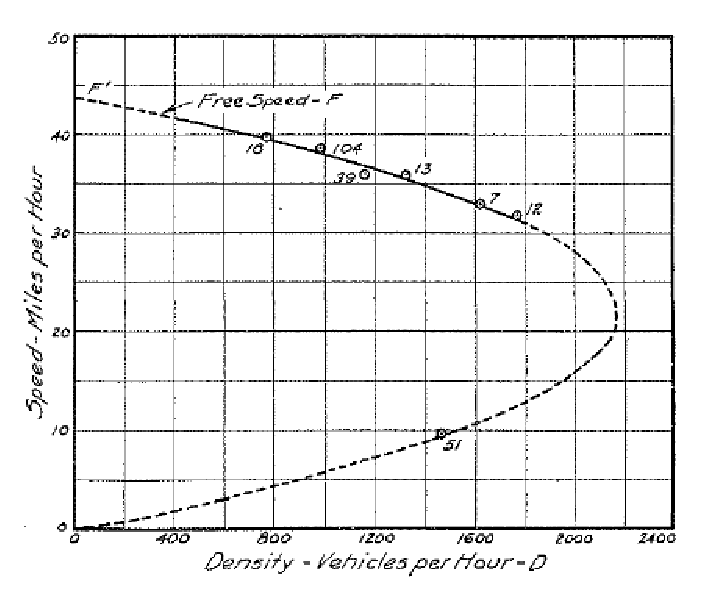
\includegraphics[scale=.75]{green.eps}
\caption{Greenshields' traffic model, reprinted from [Greenshields et al. 1935]. As shown, it is difficult to determine traffic speed from traffic flow, hence the use of flow data for validation of traffic speeds instead of determination.}
\end{figure}

\subsection{Optimal route}
In order to determine the best possible taxi ride in Manhattan, we need to consider cost, time, and path simultaneously.  Optimal path is a straightforward problem when considering only distance---any effective search algorithm will suffice (we are using A* search).  When considering time, it becomes necessary to estimate the effect of traffic on taxi speed.  Highly congested roads should not carry the same weight per distance as clear roads of the same length.
\subsection{Suboptimal routes}
The theoretical suboptimality of a route (at a given time) is determined by subtracting the expected time (or fare) of the optimal route from that of the suboptimal route. Actual time is not used as it has the undesirable property of being dependent on factors outside of the driver's control (such as red lights). The suboptimal route itself can be found from the distance traveled by the taxi via Yen's k shortest loopless paths algorithm\cite{yen}.

\section{Implementation}
\begin{figure*}
\centering
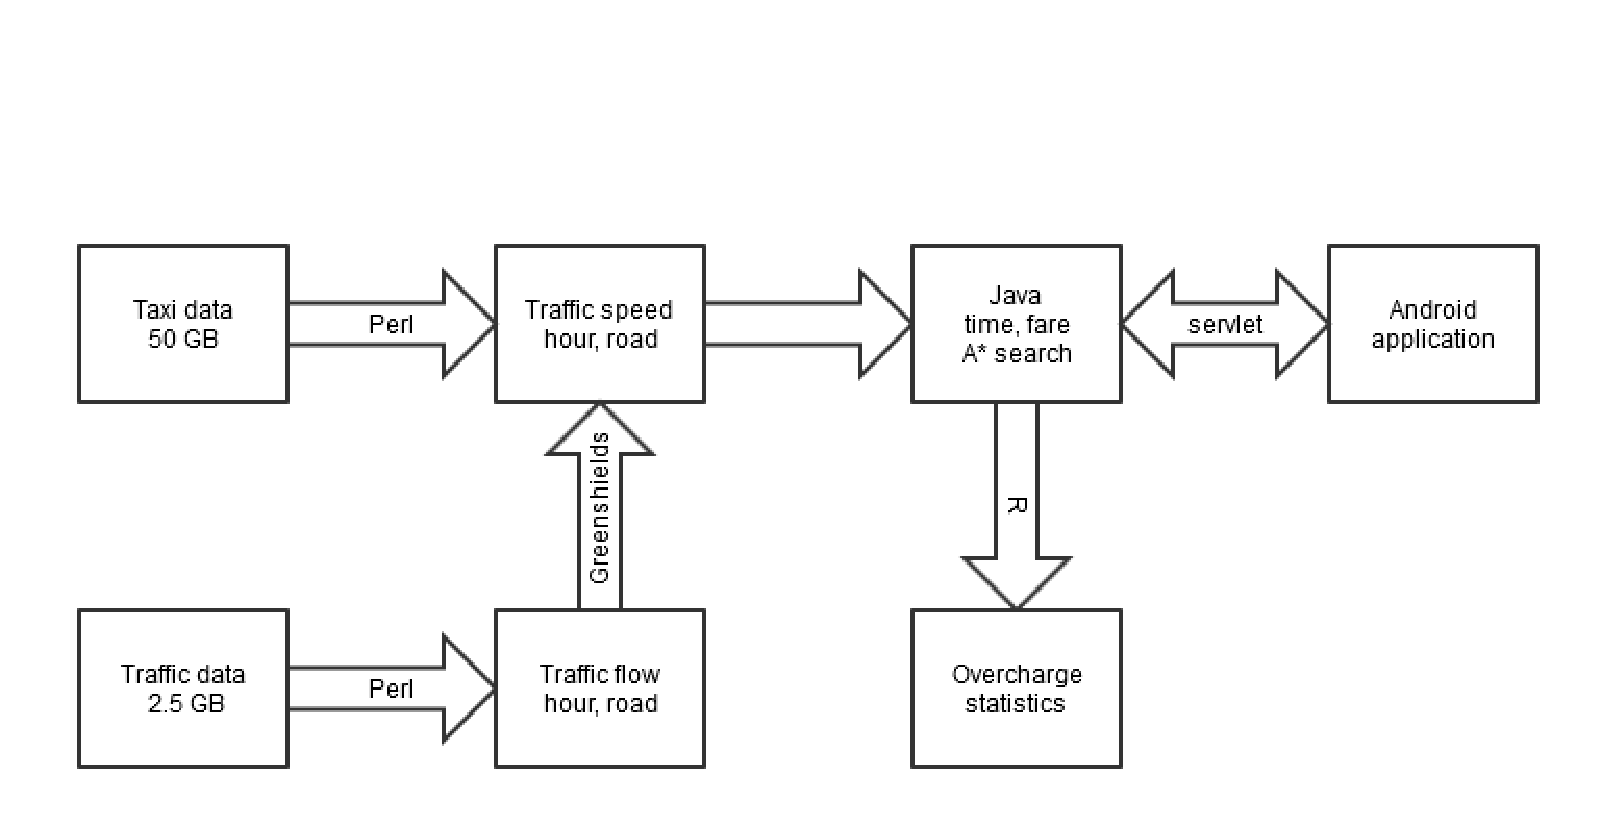
\includegraphics[scale=.60]{traffic.eps}
\caption{Summary of implementation details}
\end{figure*}
Analysis of the raw data will primarily take place using Perl via cron jobs on a Linux server. Java and R will also be used for finding the optimal path and determining if taxi drivers overcharge, respectively.  All code will be available under the MIT license on a public github repository\cite{git}. Once the models are constructed, they will be implemented into a Java servlet that will provide the Android application with the estimated time and fare for the taxi trip.
\subsection{Traffic speed model}
For the traffic speed model, taxi trips along a single road will be used to determine the speed on that road (by dividing the distance traveled by the taxi over the time of the trip). For trips that span two roads, the calculation is slightly more complicated. By assuming the model derived from only including trips along a single road is reasonably accurate, the speed along each road can be estimated, assuming data exists for both roads in the initial model, by multiplying the speed predicted by the initial model by factor
\begin{displaymath}k=\frac{t}{v_{1}\times d_{1}+v_{2}\times d_{2}}\end{displaymath}
where t is the total time, v\textsubscript{1} is the predicted speed along the first road, d\textsubscript{1} is the distance traveled along the first road, v\textsubscript{2} is the predicted speed along the second road, and d\textsubscript{2} is the distance traveled along the second road. If this data does not exist for one or both of the roads, the traffic on the two roads is assumed to be the same, so that the speed on each is just the total distance divided by the total time. Naturally, the traffic speed model is only updated at the end of the iteration involving two roads to prevent error amplification.

This process continues up to trips involving n roads, where n is around five, with the model updated at end of each iteration. Of course, as n increases, so does inherent error in the determination of road speeds and the chance of encountering an ambiguous route in which there exist multiple paths from the starting point to the destination that all cover roughly the same number of miles. These ambiguous routes are ignored. Since n is fairly small, routes can be found via a brute force search on the road graph without too much overhead.

For trips spanning n roads, the predicted speed is multiplied by factor
\begin{displaymath}
k=\frac{t}{\sum\limits_{i=1}^n v_{i}\times d_{i}}
\end{displaymath}
where v\textsubscript{i} is the predicted speed along road i and d\textsubscript{i} is the distance traveled along this road. If at any point a road does not have a predicted speed, this road will be assigned a predicted speed equal to the average of the speeds of all the other roads that do have predicted speeds, or 1 if none of the roads have predicted speeds. This is not expected to occur given that around fifty gigabytes of taxi data are available for analysis.

Although only the final iteration predictive model will be used for subsequent steps, it will be compared to the initial model to make sure errors are not amplified at each step. If error amplification proves to be a problem, an earlier iteration or even the initial one can be used for the predictive model. In this case, the traffic flow data can also help fill in any gaps.

\subsection{Traffic flow model}
For the traffic flow model, the RC\_ID of each station is mapped to the corresponding road on the graph. This, along with the FHWA direction code, allows the traffic flow data to be overlayed onto the road graph and compared with the traffic speed model. Traffic is not grouped by lane.

\subsection{Optimal path}
In order to determine the optimal path from one location in Manhattan to another, we are using A* search on a directed graph that we will create using the streets in Manhattan.  We are using an adjacency matrix to hold the graph data.  Every street crossing acts as a node on the graph.  In order to determine the weights of the edges on the graph, we plan to use a combination of traffic data for individual streets in Manhattan as well as the distance from one street to another. The traffic data is not necessary for simply determining the shortest distance, as that would be literally the "Manhattan distance" from one point to another.  By using the traffic data, however, the search should be more accurate, useful, and interesting.

We are using Java to implement the search algorithm and adjacency matrix.  We are not sure if we are going to perform the search function on a client device or on a server.  We will not need to significantly change the code regardless of whichever direction we go.  The only added consideration will be network communication.  Although the traffic data is extremely large, the results of our analysis should be relatively small, meaning that our data for estimated traffic should be able to fit on a mobile device.  Once that data takes shape, it will be easy to associate it with an edge of the graph by storing the data in a dedicated object.  Said object can then be stored in the adjacency matrix for every edge on the graph.

The rationale for using Java is twofold.  Firstly, the student implementing this part is more comfortable with Java than other languages that could perform the same functions.  Secondly, because we plan to package the end product in an Android mobile application, using Java should make it easy to perform any interfacing or communication that is necessary between backend and frontend code.

Determining the optimal path will give the user a great deal of information.  Because we have historic traffic data, we are confident that we can reasonably predict traffic congestion.  In turn, we are confident that we can reasonably predict the average speed of a taxi taking the path that is found to be optimal given our data.  Armed with this information, we can use the optimal path to give the user what should be a fairly accurate estimate for travel time.  While there are multiple variables that determine the cost of a ride, the principle determinants are time and distance.  This means that a fairly accurate estimate for cost follows from the time estimate and the distance returned from our search.

%end

\subsection{Android application}
The Android application will use the location API to determine the user's location, the start point of the trip. Once the end address is entered in, the application will send the two address to the Java servlet. The servlet will return the estimated distance, time and fare of the trip. The application will then relay this information to the user. It will also show the rates of alternative methods of transportation (such as subway) for comparison purposes.

\subsection{Overcharge statistics}
R will be used in conjunction with Perl and the Java program to determine how often and how much taxi drivers are overcharging based on the time of day. A Perl script will parse the taxi data and use the Java program to find the optimal route. Naturally, the Perl script will be run via a cron job on a remote server. If this optimal route differs from that of the route taken by the taxi and the difference in the theoretical duration of the suboptimal route compared to the optimal one is above a certain threshold, the difference in theoretical duration and fare will be recorded to a file. The difference in the actual duration and fare of the taxi route compared to the optimal route will also be recorded to a different file, regardless of whether or not the taxi route is optimal. R will then parse these files and plot the frequency of the theoretical overcharges and mean theoretical overcharge at each hour of the day, along with the actual mean overcharge or undercharge at that hour. Additionally, R will check if taxis taking optimal routes run the meters, resulting in longer than expected times or higher than expected rates showing up in the data.

\section{Results}
Traffic flow is highly variable based on time of day and road. However, even accounting for these factors there is still a substantial amount of variation. Depending on the variability of the traffic speed data, the introduction of additional variables such as day of week or season to the traffic speed prediction model might be merited. Statistical tests such as ANOVA can be used to evaluate the accuracy of the traffic speed model. The flow data can also help corroborate the model and make sure the taxis are not driving slower than regular traffic.

\section{Related Work}
There exist Android apps that estimate the taxi fare (such as Taxi-Calculator). However, these applications do not reveal how the fare is calculated or use the same data as our application. By focusing exclusively on New York and incorporating over ten gigabytes of taxi data into our model, we hope that our application will be able to outperform the existing applications. Additionally, by making our algorithms public, other researchers will be able to further improve the code.

\section{Conclusion}
Most of the groundwork for the Android application has been laid out. Future steps include finishing the road graph, analyzing the taxi data, determining if taxi drivers are overcharging, and coding up the Android application.

% The following two commands are all you need in the
% initial runs of your .tex file to
% produce the bibliography for the citations in your paper.
\bibliographystyle{abbrv}
\bibliography{cite.bib}
% sigproc.bib is the name of the Bibliography in this case
% You must have a proper ".bib" file
%  and remember to run:
% latex bibtex latex latex
% to resolve all references
%
% ACM needs 'a single self-contained file'!
%
%APPENDICES are optional
%\balancecolumns
%\balancecolumns % GM June 2007
% That's all folks!
\end{document}
